\documentclass{article}
\usepackage{minted}
\usepackage{graphicx}
\usepackage{amsmath}
\usepackage{fancyhdr}
\usepackage{hyperref}
\usepackage[dvipsnames]{xcolor}
\usepackage{enumitem}
\usepackage{minted}
\usepackage{minted}
%%%%% NEW MATH DEFINITIONS %%%%%

\usepackage{amsmath,amsfonts,bm,bbm}

\def\ind{{\mathbbm{1}}}

% Mark sections of captions for referring to divisions of figures
\newcommand{\figleft}{{\em (Left)}}
\newcommand{\figcenter}{{\em (Center)}}
\newcommand{\figright}{{\em (Right)}}
\newcommand{\figtop}{{\em (Top)}}
\newcommand{\figbottom}{{\em (Bottom)}}
\newcommand{\captiona}{{\em (a)}}
\newcommand{\captionb}{{\em (b)}}
\newcommand{\captionc}{{\em (c)}}
\newcommand{\captiond}{{\em (d)}}
\newcommand{\figleftt}{{\em Left}}
\newcommand{\figcentert}{{\em Center}}
\newcommand{\figrightt}{{\em Right}}
\newcommand{\figtopt}{{\em Top}}
\newcommand{\figbottomt}{{\em Bottom}}
\newcommand{\captionat}{{\em a}}
\newcommand{\captionbt}{{\em b}}
\newcommand{\captionct}{{\em c}}
\newcommand{\captiondt}{{\em d}}

% Highlight a newly defined term
\newcommand{\newterm}[1]{{\bf #1}}


% Figure reference, lower-case.
\def\figref#1{figure~\ref{#1}}
% Figure reference, capital. For start of sentence
\def\Figref#1{Figure~\ref{#1}}
\def\twofigref#1#2{figures \ref{#1} and \ref{#2}}
\def\quadfigref#1#2#3#4{figures \ref{#1}, \ref{#2}, \ref{#3} and \ref{#4}}
% Section reference, lower-case.
\def\secref#1{section~\ref{#1}}
% Section reference, capital.
\def\Secref#1{Section~\ref{#1}}
% Reference to two sections.
\def\twosecrefs#1#2{sections \ref{#1} and \ref{#2}}
% Reference to three sections.
\def\secrefs#1#2#3{sections \ref{#1}, \ref{#2} and \ref{#3}}

\def\chapref#1{chapter~\ref{#1}}
% Reference to an equation, upper case.
\def\Chapref#1{Chapter~\ref{#1}}
% Reference to a range of chapters
\def\rangechapref#1#2{chapters\ref{#1}--\ref{#2}}
% Reference to an algorithm, lower-case.
\def\algref#1{algorithm~\ref{#1}}
% Reference to an algorithm, upper case.
\def\Algref#1{Algorithm~\ref{#1}}
\def\twoalgref#1#2{algorithms \ref{#1} and \ref{#2}}
\def\Twoalgref#1#2{Algorithms \ref{#1} and \ref{#2}}
% Reference to a part, lower case
\def\partref#1{part~\ref{#1}}
% Reference to a part, upper case
\def\Partref#1{Part~\ref{#1}}
\def\twopartref#1#2{parts \ref{#1} and \ref{#2}}

\def\ceil#1{\lceil #1 \rceil}
\def\floor#1{\lfloor #1 \rfloor}
\def\1{\bm{1}}
\newcommand{\train}{\mathcal{D}}
\newcommand{\valid}{\mathcal{D_{\mathrm{valid}}}}
\newcommand{\test}{\mathcal{D_{\mathrm{test}}}}

\def\eps{{\epsilon}}


% Random variables
\def\reta{{\textnormal{$\eta$}}}
\def\ra{{\textnormal{a}}}
\def\rb{{\textnormal{b}}}
\def\rc{{\textnormal{c}}}
\def\rd{{\textnormal{d}}}
\def\re{{\textnormal{e}}}
\def\rf{{\textnormal{f}}}
\def\rg{{\textnormal{g}}}
\def\rh{{\textnormal{h}}}
\def\ri{{\textnormal{i}}}
\def\rj{{\textnormal{j}}}
\def\rk{{\textnormal{k}}}
\def\rl{{\textnormal{l}}}
% rm is already a command, just don't name any random variables m
\def\rn{{\textnormal{n}}}
\def\ro{{\textnormal{o}}}
\def\rp{{\textnormal{p}}}
\def\rq{{\textnormal{q}}}
\def\rr{{\textnormal{r}}}
\def\rs{{\textnormal{s}}}
\def\rt{{\textnormal{t}}}
\def\ru{{\textnormal{u}}}
\def\rv{{\textnormal{v}}}
\def\rw{{\textnormal{w}}}
\def\rx{{\textnormal{x}}}
\def\ry{{\textnormal{y}}}
\def\rz{{\textnormal{z}}}

% Random vectors
\def\rvepsilon{{\mathbf{\epsilon}}}
\def\rvtheta{{\mathbf{\theta}}}
\def\rva{{\mathbf{a}}}
\def\rvb{{\mathbf{b}}}
\def\rvc{{\mathbf{c}}}
\def\rvd{{\mathbf{d}}}
\def\rve{{\mathbf{e}}}
\def\rvf{{\mathbf{f}}}
\def\rvg{{\mathbf{g}}}
\def\rvh{{\mathbf{h}}}
\def\rvu{{\mathbf{i}}}
\def\rvj{{\mathbf{j}}}
\def\rvk{{\mathbf{k}}}
\def\rvl{{\mathbf{l}}}
\def\rvm{{\mathbf{m}}}
\def\rvn{{\mathbf{n}}}
\def\rvo{{\mathbf{o}}}
\def\rvp{{\mathbf{p}}}
\def\rvq{{\mathbf{q}}}
\def\rvr{{\mathbf{r}}}
\def\rvs{{\mathbf{s}}}
\def\rvt{{\mathbf{t}}}
\def\rvu{{\mathbf{u}}}
\def\rvv{{\mathbf{v}}}
\def\rvw{{\mathbf{w}}}
\def\rvx{{\mathbf{x}}}
\def\rvy{{\mathbf{y}}}
\def\rvz{{\mathbf{z}}}

% Elements of random vectors
\def\erva{{\textnormal{a}}}
\def\ervb{{\textnormal{b}}}
\def\ervc{{\textnormal{c}}}
\def\ervd{{\textnormal{d}}}
\def\erve{{\textnormal{e}}}
\def\ervf{{\textnormal{f}}}
\def\ervg{{\textnormal{g}}}
\def\ervh{{\textnormal{h}}}
\def\ervi{{\textnormal{i}}}
\def\ervj{{\textnormal{j}}}
\def\ervk{{\textnormal{k}}}
\def\ervl{{\textnormal{l}}}
\def\ervm{{\textnormal{m}}}
\def\ervn{{\textnormal{n}}}
\def\ervo{{\textnormal{o}}}
\def\ervp{{\textnormal{p}}}
\def\ervq{{\textnormal{q}}}
\def\ervr{{\textnormal{r}}}
\def\ervs{{\textnormal{s}}}
\def\ervt{{\textnormal{t}}}
\def\ervu{{\textnormal{u}}}
\def\ervv{{\textnormal{v}}}
\def\ervw{{\textnormal{w}}}
\def\ervx{{\textnormal{x}}}
\def\ervy{{\textnormal{y}}}
\def\ervz{{\textnormal{z}}}

% Random matrices
\def\rmA{{\mathbf{A}}}
\def\rmB{{\mathbf{B}}}
\def\rmC{{\mathbf{C}}}
\def\rmD{{\mathbf{D}}}
\def\rmE{{\mathbf{E}}}
\def\rmF{{\mathbf{F}}}
\def\rmG{{\mathbf{G}}}
\def\rmH{{\mathbf{H}}}
\def\rmI{{\mathbf{I}}}
\def\rmJ{{\mathbf{J}}}
\def\rmK{{\mathbf{K}}}
\def\rmL{{\mathbf{L}}}
\def\rmM{{\mathbf{M}}}
\def\rmN{{\mathbf{N}}}
\def\rmO{{\mathbf{O}}}
\def\rmP{{\mathbf{P}}}
\def\rmQ{{\mathbf{Q}}}
\def\rmR{{\mathbf{R}}}
\def\rmS{{\mathbf{S}}}
\def\rmT{{\mathbf{T}}}
\def\rmU{{\mathbf{U}}}
\def\rmV{{\mathbf{V}}}
\def\rmW{{\mathbf{W}}}
\def\rmX{{\mathbf{X}}}
\def\rmY{{\mathbf{Y}}}
\def\rmZ{{\mathbf{Z}}}
\def\rmtheta{{\mathbf{\Theta}}}
% Elements of random matrices
\def\ermA{{\textnormal{A}}}
\def\ermB{{\textnormal{B}}}
\def\ermC{{\textnormal{C}}}
\def\ermD{{\textnormal{D}}}
\def\ermE{{\textnormal{E}}}
\def\ermF{{\textnormal{F}}}
\def\ermG{{\textnormal{G}}}
\def\ermH{{\textnormal{H}}}
\def\ermI{{\textnormal{I}}}
\def\ermJ{{\textnormal{J}}}
\def\ermK{{\textnormal{K}}}
\def\ermL{{\textnormal{L}}}
\def\ermM{{\textnormal{M}}}
\def\ermN{{\textnormal{N}}}
\def\ermO{{\textnormal{O}}}
\def\ermP{{\textnormal{P}}}
\def\ermQ{{\textnormal{Q}}}
\def\ermR{{\textnormal{R}}}
\def\ermS{{\textnormal{S}}}
\def\ermT{{\textnormal{T}}}
\def\ermU{{\textnormal{U}}}
\def\ermV{{\textnormal{V}}}
\def\ermW{{\textnormal{W}}}
\def\ermX{{\textnormal{X}}}
\def\ermY{{\textnormal{Y}}}
\def\ermZ{{\textnormal{Z}}}

% Vectors
\def\vzero{{\bm{0}}}
\def\vone{{\bm{1}}}
\def\vmu{{\bm{\mu}}}
\def\vtheta{{\bm{\theta}}}
\def\va{{\bm{a}}}
\def\vb{{\bm{b}}}
\def\vc{{\bm{c}}}
\def\vd{{\bm{d}}}
\def\ve{{\bm{e}}}
\def\vf{{\bm{f}}}
\def\vg{{\bm{g}}}
\def\vh{{\bm{h}}}
\def\vi{{\bm{i}}}
\def\vj{{\bm{j}}}
\def\vk{{\bm{k}}}
\def\vl{{\bm{l}}}
\def\vm{{\bm{m}}}
\def\vn{{\bm{n}}}
\def\vo{{\bm{o}}}
\def\vp{{\bm{p}}}
\def\vq{{\bm{q}}}
\def\vr{{\bm{r}}}
\def\vs{{\bm{s}}}
\def\vt{{\bm{t}}}
\def\vu{{\bm{u}}}
\def\vv{{\bm{v}}}
\def\vw{{\bm{w}}}
\def\vx{{\bm{x}}}
\def\vy{{\bm{y}}}
\def\vz{{\bm{z}}}

% Elements of vectors
\def\evalpha{{\alpha}}
\def\evbeta{{\beta}}
\def\evepsilon{{\epsilon}}
\def\evlambda{{\lambda}}
\def\evomega{{\omega}}
\def\evmu{{\mu}}
\def\evpsi{{\psi}}
\def\evsigma{{\sigma}}
\def\evtheta{{\theta}}
\def\eva{{a}}
\def\evb{{b}}
\def\evc{{c}}
\def\evd{{d}}
\def\eve{{e}}
\def\evf{{f}}
\def\evg{{g}}
\def\evh{{h}}
\def\evi{{i}}
\def\evj{{j}}
\def\evk{{k}}
\def\evl{{l}}
\def\evm{{m}}
\def\evn{{n}}
\def\evo{{o}}
\def\evp{{p}}
\def\evq{{q}}
\def\evr{{r}}
\def\evs{{s}}
\def\evt{{t}}
\def\evu{{u}}
\def\evv{{v}}
\def\evw{{w}}
\def\evx{{x}}
\def\evy{{y}}
\def\evz{{z}}

% Matrix
\def\mA{{\bm{A}}}
\def\mB{{\bm{B}}}
\def\mC{{\bm{C}}}
\def\mD{{\bm{D}}}
\def\mE{{\bm{E}}}
\def\mF{{\bm{F}}}
\def\mG{{\bm{G}}}
\def\mH{{\bm{H}}}
\def\mI{{\bm{I}}}
\def\mJ{{\bm{J}}}
\def\mK{{\bm{K}}}
\def\mL{{\bm{L}}}
\def\mM{{\bm{M}}}
\def\mN{{\bm{N}}}
\def\mO{{\bm{O}}}
\def\mP{{\bm{P}}}
\def\mQ{{\bm{Q}}}
\def\mR{{\bm{R}}}
\def\mS{{\bm{S}}}
\def\mT{{\bm{T}}}
\def\mU{{\bm{U}}}
\def\mV{{\bm{V}}}
\def\mW{{\bm{W}}}
\def\mX{{\bm{X}}}
\def\mY{{\bm{Y}}}
\def\mZ{{\bm{Z}}}
\def\mBeta{{\bm{\beta}}}
\def\mPhi{{\bm{\Phi}}}
\def\mLambda{{\bm{\Lambda}}}
\def\mSigma{{\bm{\Sigma}}}

% Tensor
\DeclareMathAlphabet{\mathsfit}{\encodingdefault}{\sfdefault}{m}{sl}
\SetMathAlphabet{\mathsfit}{bold}{\encodingdefault}{\sfdefault}{bx}{n}
\newcommand{\tens}[1]{\bm{\mathsfit{#1}}}
\def\tA{{\tens{A}}}
\def\tB{{\tens{B}}}
\def\tC{{\tens{C}}}
\def\tD{{\tens{D}}}
\def\tE{{\tens{E}}}
\def\tF{{\tens{F}}}
\def\tG{{\tens{G}}}
\def\tH{{\tens{H}}}
\def\tI{{\tens{I}}}
\def\tJ{{\tens{J}}}
\def\tK{{\tens{K}}}
\def\tL{{\tens{L}}}
\def\tM{{\tens{M}}}
\def\tN{{\tens{N}}}
\def\tO{{\tens{O}}}
\def\tP{{\tens{P}}}
\def\tQ{{\tens{Q}}}
\def\tR{{\tens{R}}}
\def\tS{{\tens{S}}}
\def\tT{{\tens{T}}}
\def\tU{{\tens{U}}}
\def\tV{{\tens{V}}}
\def\tW{{\tens{W}}}
\def\tX{{\tens{X}}}
\def\tY{{\tens{Y}}}
\def\tZ{{\tens{Z}}}


% Graph
\def\gA{{\mathcal{A}}}
\def\gB{{\mathcal{B}}}
\def\gC{{\mathcal{C}}}
\def\gD{{\mathcal{D}}}
\def\gE{{\mathcal{E}}}
\def\gF{{\mathcal{F}}}
\def\gG{{\mathcal{G}}}
\def\gH{{\mathcal{H}}}
\def\gI{{\mathcal{I}}}
\def\gJ{{\mathcal{J}}}
\def\gK{{\mathcal{K}}}
\def\gL{{\mathcal{L}}}
\def\gM{{\mathcal{M}}}
\def\gN{{\mathcal{N}}}
\def\gO{{\mathcal{O}}}
\def\gP{{\mathcal{P}}}
\def\gQ{{\mathcal{Q}}}
\def\gR{{\mathcal{R}}}
\def\gS{{\mathcal{S}}}
\def\gT{{\mathcal{T}}}
\def\gU{{\mathcal{U}}}
\def\gV{{\mathcal{V}}}
\def\gW{{\mathcal{W}}}
\def\gX{{\mathcal{X}}}
\def\gY{{\mathcal{Y}}}
\def\gZ{{\mathcal{Z}}}

% Sets
\def\sA{{\mathbb{A}}}
\def\sB{{\mathbb{B}}}
\def\sC{{\mathbb{C}}}
\def\sD{{\mathbb{D}}}
% Don't use a set called E, because this would be the same as our symbol
% for expectation.
\def\sF{{\mathbb{F}}}
\def\sG{{\mathbb{G}}}
\def\sH{{\mathbb{H}}}
\def\sI{{\mathbb{I}}}
\def\sJ{{\mathbb{J}}}
\def\sK{{\mathbb{K}}}
\def\sL{{\mathbb{L}}}
\def\sM{{\mathbb{M}}}
\def\sN{{\mathbb{N}}}
\def\sO{{\mathbb{O}}}
\def\sP{{\mathbb{P}}}
\def\sQ{{\mathbb{Q}}}
\def\sR{{\mathbb{R}}}
\def\sS{{\mathbb{S}}}
\def\sT{{\mathbb{T}}}
\def\sU{{\mathbb{U}}}
\def\sV{{\mathbb{V}}}
\def\sW{{\mathbb{W}}}
\def\sX{{\mathbb{X}}}
\def\sY{{\mathbb{Y}}}
\def\sZ{{\mathbb{Z}}}

% Entries of a matrix
\def\emLambda{{\Lambda}}
\def\emA{{A}}
\def\emB{{B}}
\def\emC{{C}}
\def\emD{{D}}
\def\emE{{E}}
\def\emF{{F}}
\def\emG{{G}}
\def\emH{{H}}
\def\emI{{I}}
\def\emJ{{J}}
\def\emK{{K}}
\def\emL{{L}}
\def\emM{{M}}
\def\emN{{N}}
\def\emO{{O}}
\def\emP{{P}}
\def\emQ{{Q}}
\def\emR{{R}}
\def\emS{{S}}
\def\emT{{T}}
\def\emU{{U}}
\def\emV{{V}}
\def\emW{{W}}
\def\emX{{X}}
\def\emY{{Y}}
\def\emZ{{Z}}
\def\emSigma{{\Sigma}}

% entries of a tensor
% Same font as tensor, without \bm wrapper
\newcommand{\etens}[1]{\mathsfit{#1}}
\def\etLambda{{\etens{\Lambda}}}
\def\etA{{\etens{A}}}
\def\etB{{\etens{B}}}
\def\etC{{\etens{C}}}
\def\etD{{\etens{D}}}
\def\etE{{\etens{E}}}
\def\etF{{\etens{F}}}
\def\etG{{\etens{G}}}
\def\etH{{\etens{H}}}
\def\etI{{\etens{I}}}
\def\etJ{{\etens{J}}}
\def\etK{{\etens{K}}}
\def\etL{{\etens{L}}}
\def\etM{{\etens{M}}}
\def\etN{{\etens{N}}}
\def\etO{{\etens{O}}}
\def\etP{{\etens{P}}}
\def\etQ{{\etens{Q}}}
\def\etR{{\etens{R}}}
\def\etS{{\etens{S}}}
\def\etT{{\etens{T}}}
\def\etU{{\etens{U}}}
\def\etV{{\etens{V}}}
\def\etW{{\etens{W}}}
\def\etX{{\etens{X}}}
\def\etY{{\etens{Y}}}
\def\etZ{{\etens{Z}}}


\DeclareMathOperator{\E}{\mathbb{E}}
\newcommand{\Ls}{\mathcal{L}}
\newcommand{\R}{\mathbb{R}}
\newcommand{\emp}{\tilde{p}}
\newcommand{\lr}{\alpha}
\newcommand{\reg}{\lambda}
\newcommand{\sigmoid}{\sigma}
\newcommand{\softplus}{\zeta}
\newcommand{\KL}{D_{\mathrm{KL}}}
\newcommand{\Var}{\mathrm{Var}}
\newcommand{\standarderror}{\mathrm{SE}}
\newcommand{\Cov}{\mathrm{Cov}}
\DeclareMathOperator*{\argmax}{arg\,max}
\DeclareMathOperator*{\argmin}{arg\,min}

\DeclareMathOperator{\sign}{sign}
\DeclareMathOperator{\Tr}{Tr}
\let\ab\allowbreak

\newcommand{\vbar}[1]{\bigg\rvert_{#1}}
\newcommand\at[2]{\left.#1\right|_{#2}}
\newcommand{\bs}[1]{\boldsymbol{#1}}

\newcommand{\sigx}[1]{\sigma_{x,#1}}
\newcommand{\sigb}[1]{\sigma_{\beta,#1}}

\newcommand{\dd}{\mathrm{d}} %for integration

\newcommand{\bb}{b}

\pagestyle{empty} \addtolength{\textwidth}{1.0in}
\addtolength{\textheight}{0.5in} \addtolength{\oddsidemargin}{-0.5in}
\addtolength{\evensidemargin}{0.5in}
\newcommand{\ruleskip}{\bigskip\hrule\bigskip}
\newcommand{\nodify}[1]{{\sc #1}} \newcommand{\points}[1]{{\textbf{[#1
points]}}}

\newcommand{\bitem}{\begin{list}{$\bullet$}%
{\setlength{\itemsep}{0pt}\setlength{\topsep}{0pt}%
\setlength{\rightmargin}{0pt}}} \newcommand{\eitem}{\end{list}}

\definecolor{nyupurple}{RGB}{134, 0, 179}
\setlength{\parindent}{0pt} \setlength{\parskip}{0.5ex}

\begin{document}

\pagestyle{myheadings} \markboth{}{\color{nyupurple} DS-GA-1003 - Spring 2023}

\begin{center}
{\Large
Homework 1: Error Decomposition \& Polynomial Regression
} 
\end{center}

{
{ \color{nyupurple} \textbf{Due:} Wednesday, February 1, 2023 at 11:59pm} 
} 

\textbf{Instructions: }Your answers to the questions below, including plots and mathematical
 work, should be submitted as a single PDF file.  It's preferred that you write your answers using software that typesets mathematics (e.g.LaTeX, LyX, or MathJax via iPython), though if you need to you may scan handwritten work.  You may find the \href{https://github.com/gpoore/minted}{minted} package convenient for including source code in your LaTeX document.  If you are using LyX, then the \href{https://en.wikibooks.org/wiki/LaTeX/Source_Code_Listings}{listings} package tends to work better. The last application is optional. 

 \ruleskip

\textbf{\color{nyupurple} General considerations (10 Points)}

For the first part of this assignment we will consider a synthetic prediction problem to develop our intuition about the error decomposition. Consider the random variables $x \in \mathcal{X} = [0,1]$ distributed uniformely ($ x \sim \mathrm{Unif}([0,1])$) and $y \in \mathcal{Y} = \sR$ defined as a polynomial of degree 2 of $x$: there exists $(a_0, a_1, a_2) \in \sR^3$ such that the values of $x$ and $y$ are linked as $y = g(x) = a_0 + a_1 x + a_2 x^2$. Note that this relation fixes the joint distribution $P_{\mathcal{X} \times \mathcal{Y}}$.

From the knowledge of a sample $\{x_i, y_i\}_{i=1}^N$, we would like to predict the relation between $x$ and $y$, that is find a function $f$ to make predictions $\hat{y} = f(x)$. We note $\gH_d$, the set of polynomial functions on $\R$ of degree $d$: $\gH_d = \left\{f: x \rightarrow \bb_0 + \bb x + \cdots \bb_d x^d; \bb_k \in \sR \forall k\in \{0, \cdots d\} \right\}$. We will consider the hypothesis classes $\gH_d$ varying d.
We will minimize the squared loss $\ell(\hat{y},y) = \frac 1 2 (\hat{y} - y)^2$ to solve the regression problem.

\newcounter{saveenum}
\begin{enumerate}
    \item (2 Points) Recall the definition of the expected risk $R(f)$ of a predictor $f$. While this cannot be computed in general note that here we defined $P_{\mathcal{X} \times \mathcal{Y}}$. Which function $f^*$ is an obvious Bayes predictor? Make sure to explain why the risk $R(f^*)$ is minimum at $f^*$.
    \begin{itemize}
        \item risk is defined as $R(f)=E_{x,y\sim P_{X\times Y}}[\ell(f(x),y)]$
        \item we know that y is a deterministic function of x, so we can set our optimal function of x as $f^{*}(x)=y=a_0+a_1x+a_2^2x$
        \item if we set $f^{*}(x)=y(x)=y$ it is clear that our predictor will equal y for any given value of x, and thus as the loss is defined as $\ell(f^{*}(x))=\frac{1}{2}(f^{*}(x)-y)=\frac{1}{2}(y(x)-y(x))^2=0$ our loss any given x will be zero. thus setting x as such we face no risk
    \end{itemize}

    
    \item (2 Points) Using $\gH_2$ as your hypothesis class, which function $f^*_{\gH_2}$ is a risk minimizer in $\gH_2$? Recall the definition of the approximation error. What is the approximation error achieved by $f^*_{\gH_2}$?

\begin{itemize}
    \item assuming my argument in the last question is correct, $f^{*}$ is within $\mathcal{H}_{2}$ thus $y=y(x)=f^{*}(x)=f^{*}_{\mathcal{H}_2}=a_0+a_1x+a_2^2x$
    \item since $f^{*}(x)=f^{*}_{\mathcal{H}_2}$ the approximation error will be zero, this makes sense as by restraining our selves to polynomials of degree two we do not lose any accuracy.
\end{itemize}

    
    \item (2 Points) Considering now $\gH_d$, with $d>2$. Justify an inequality between $R(f^*_{\gH_2})$ and $R(f^*_{\gH_d})$. Which function $f^*_{\gH_d}$ is a risk minimizer in $\gH_d$? What is the approximation error achieved by $f^*_{\gH_d}$?

    \begin{itemize}
    \item due to the fact that $f^{*}(x)=f^{*}_{\mathcal{H}_2}$ by definition of Bayes risk, it must be the case that $R(f^*_{\gH_2})\leq R(f^*_{\gH_d})$
    \item we don't have any restrictions on the values of the constants, so by the same argument as in question one we could pick $f^*_{\gH_d}=a_0+a_1x+a_2x^2+0x^3+0x^4...+0x^d$ that is we set $b_{i}=0\forall i \in [3,d]$
    \item further as $f^*_{\gH_d}=a_0+a_1x+a_2x^2+0x^3+0x^4...+0x^d=a_0+a_1x+a_2^2x=f^*_{\gH_2}=f^{*}(x)=y(x)=y$ by the same argument as part 2 there is no approximation error
    \end{itemize}
    \item (4 Points) For this question we assume $a_0 = 0$. Considering $\gH= \left\{f: x \rightarrow \bb_1 x;  \bb_1 \in \sR\right\}$, which function $f^*_{\gH}$ is a risk minimizer in $\gH$? What is the approximation error achieved by $f^*_{\gH}$? In particular what is the approximation error achieved if furthermore $a_2=0$ in the definition of true underlying relation $g(x)$ above?


    \begin{itemize}
    \item out goal is to find a single $\alpha\in \mathbb{R}$ such that the risk is minimized. 
    \item so our problem can be expressed as $R(f_{H}^*(x))=E[\ell(f_{H}^*(x),y)]=E[\frac{1}{2}(\alpha x- a_1x-a_2x^2 )]=\frac{1}{2}E[(x(\alpha - a_1)-a_2x^2 )^2]=\int_{0}^{1}(x(\alpha - a_1)-a_2x^2 )^2P(x=x)dx=\int_{0}^{1}(x(\alpha - a_1)-a_2x^2 )^2P(x=x)dx$ by the properties of uniform random variables $\int_{0}^{1}(x(\alpha - a_1)-a_2x^2 )^2dx$ 
    \item then we can expand this as $(f_{H}^*(x))=\int_{0}^{1}(x(\alpha - a_1)-a_2x^2 )^2dx=\int_{0}^{1}\left(x\left(\alpha-a_1\right)\right)^2-2\alphax^3a_2+2x^3a_1a_2+a_2^2x^4dx=\frac{\left(\alpha-a_1\right)^2}{3}-\frac{\alpha a_2}{2}+\frac{a_1a_2}{2}+\frac{a_2^2}{5}$
    \item our goal is to minimize this function so we can take the derivative $\frac{\partial R}{\partial \alpha}=\frac{2\alpha -2a_1}{3}-\frac{a_2}{2}$
    \item we can take the second derivative $\frac{\partial R^2}{\partial^2 \alpha}=\frac{2}{3}\geq 0$ meaning our risk function is convex and thus any min will be a global minima 
    \item then setting our first derivative with respect to $\alpha$ equal to zero and solving for $\alpha$ yields $\alpha*=a_1+\frac{3}{4}a_2$
    \item in the case where $a_2=0$ and we set $\alpha=\alpha^*$ we can see that our risk will be $R(f_{H}^*(x))=E[\ell(f_{H}^*(x),y)]=E[\frac{1}{2}(\alpha^{*} x- a_1x-a_2x^2 )^2]=E[\frac{1}{2}((a_1+\frac{3}{4}a_2) x- a_1x-a_2x^2 )^2]=\frac{1}{2}E[(a_1 x- a_1x )^2=0$ meaning that our risk will be zero if $a_2=0$
    \end{itemize}

\setcounter{saveenum}{\value{enumi}}
\end{enumerate}

\textbf{\color{nyupurple} Polynomial regression as linear least squares (5 Points)}\\
In practice, $P_{\mathcal{X} \times \mathcal{Y}}$ is usually unknown and we use the empirical risk minimizer (ERM). We will reformulate the problem as a $d$-dimensional linear regression problem. 
First note that functions in $\gH_d$ are parametrized by a vector $\bs \bb = [\bb_0, \bb_1, \cdots \bb_d]^\top$, we will use the notation $f_{\bs \bb}$. Similarly we will note $\bs a \in \sR^3$ the vector parametrizing $g(x) = f_{\bs a}(x)$. We will also gather data points from the training sample in the following matrix and vector:
\begin{align}
    X = \left[\begin{matrix}
    1 & x_1 & \cdots & x_1^d \\
    1 & x_2 & \cdots & x_2^d \\
    \vdots & \vdots & \vdots & \vdots \\
    1 & x_N & \cdots & x_N
\end{matrix} \right], \quad 
\bs y = [y_0, y_1, \cdots y_N]^\top.
\end{align}
These notations allow us to take advantage of the very effective linear algebra formalism. $X$ is called the design matrix.
\begin{enumerate}
\setcounter{enumi}{\value{saveenum}}
    \item (2 Points) Show that the empirical risk minimizer (ERM) $\hat{\bs \bb}$ is given by the following minimization $\hat{\bs \bb} = \underset{\bb}{\arg\min}\lVert X\bb - \bs y \Vert_2^2$ .

    \begin{itemize}
        \item for simplicity think of $x_i$ as the ith row of matrix $X$ so $x_i b$ is the vector product of the ith row of x times the matrix b
        \item so it is worth noting for any given data point $f(x_i)=bx_i$
        \item empirical risk is defined as $\frac{1}{n}\Sigma_{i=1}^{n}\ell (f(x_i),y_i)$ using the loss function above this is more specifically $\frac{1}{n}\Sigma_{i=1}^{n}\ell (f(x_i),y_i)=\frac{1}{2n}\Sigma_{i=1}^{n}(f(x_i)-y_i)^2$
        \item using the l2 norm we can write $||Xb-y||_{2}=\sqrt{\Sigma_{i=1}^{n}(bx_i-y_i)^2}$ squaring this we end up with  $||Xb-y||_{2}^{2}=\Sigma_{i=1}^{n}(bx_i-y_i)^2=\Sigma_{i=1}^{n}(f(x_i)-y_i)^2$ 
        \item so note that our empirical risk and$||Xb-y||_{2}$ only differ by a constant factor $\frac{1}{2n}$ which will not effect optimization thus $\hat{b}=\underset{\bb}{\arg\min}\lVert X\bb - \bs y \Vert_2^2=\underset{f}{\arg\min}\hat{R}_{n}(f)$ which is the desired result
    \end{itemize}
    
    \item (3 Points) If $N > d$ and $X$ is full rank, show that $\hat{\bs \bb} = (X^\top X)^{-1}X^\top \bs y$. (Hint: you should take the gradients of the loss above with respect to $\bs \bb$ \footnote{You can check the linear algebra review here if needed \url{http://cs229.stanford.edu/section/cs229-linalg.pdf}}). Why do we need to use the conditions $N > d$ and $X$ full rank ?  
    \begin{itemize}
        \item we can express our question as $||Xb-y||_{2}^{2}=(Xb-y)^t(Xb-y)=(b^tX^t-y^t)(Xb-y)=b^tX^tXb-b^tX^ty-y^tXb-y^ty$
        \item now lets take its gradient in parts
        \begin{itemize}
            \item first lets consider $\frac{\partial bX^tXb}{\partial b}$ since the product of two matrices are themselves a matrix we can think of this as $\frac{\partial bX^tXb}{\partial b}=\frac{\partial b^tAb}{\partial b}$ for some matrix A which must be symmetric as it is the product of the transpose of a matrix and its self, and we know $\frac{\partial b^tAb}{\partial b}=2b^t(A)=2b^{t}(X^tX)$
            \item next we can write $\frac{\partial b^tX^ty}{\partial b}=\frac{\partial b^tv}{\partial b}=v=X^ty$
            \item then we have $\frac{\partial y^{t}Xb}{\partial b}=\frac{\partial v^{t}b}{\partial b}=v^t=y^tX$
            \item putting this all together we get $\nabla=2b^{t}(X^tX)-X^ty-y^tX=2b^{t}(X^tX)-2<X,y>$
            \item also taking the second derivative we find $\frac{\partial \nabla}{\partial b}=2X^TX$ which must be a positive definite matrix meaning the problem is convex, and thus min of our gradient will be a global min 
        \end{itemize}
        \item so now all that remains to do is to solve $\nabla=2b^{t}(X^tX)-2<X,y>=0$ this yields $b^{t}(X^{t}X)=Y^tX$ we know that X is full rank, and thus invertable.   thus we have $b^t=(y^tX)(X^{t}X)^{-1}$ then we take the transpose to finally get $b=((y^tX)(X^{t}X)^{-1})^{t}=((X^{T}X)^{-1})^t(X^{t}y)=(X^{t}X)^{-1}(X^{t}y)$ which is the desired result
        \item we need x to be full rank so that it is invertable. 
        \item we need $N>d$ since if this is not the case we are not guaranteed to have  $X^TX$ as positive semi definite, and thus the problem may not be convex meaning our solution may not be a global min. 

    \end{itemize}

    
    
\setcounter{saveenum}{\value{enumi}}  
\end{enumerate}

\textbf{\color{nyupurple} Hands on (7 Points)}\\
Open the source code file \emph{hw1\_code\_source.py} from the \emph{.zip} folder. Using the function \texttt{get\_a}  get a value for $\bs a$, and draw a sample \texttt{x\_train, y\_train} of size $N=10$ and a sample \texttt{x\_test, y\_test} of size $N_{\rm test}=1000$ using the function \texttt{draw\_sample}.

\begin{enumerate}

\setcounter{enumi}{\value{saveenum}}
    \item (2 Points) Write a function called \texttt{least\_square\_estimator} taking as input a design matrix $X \in \sR^{N \times (d + 1)}$ and the corresponding vector  $\bs y \in \sR^N$ returning $\hat{\bs b} \in \sR^{(d + 1)}$. Your function should handle any value of $N$ and $d$, and in particular return an error if $N \leq d$. (Drawing $x$ at random from the uniform distribution makes it almost certain that any design matrix $X$ with $d \geq 1$ we generate is full rank).
\inputminted[firstline=58, lastline=67, breaklines=True]{python}{hw1_code_source.py}
\begin{itemize}
\item this is a pretty direct implementation of what was derived in question 6. 

\end{itemize}

    
    \item (1 Points) Recall the definition of the empirical risk $\hat{R}(\hat{f})$ on a sample $\{x_i, y_i\}_{i=1}^N$ for a prediction function $\hat{f}$. Write a function \texttt{empirical\_risk} to compute the empirical risk of $f_{\bs \bb}$ taking as input a design matrix $X \in \sR^{N \times (d + 1)}$, a vector $\bs y \in \sR^N$ and the vector  $\bs \bb \in \sR^{(d+1)}$ parameterize the predictor.
    \inputminted[firstline=68, lastline=77, breaklines=True]{python}{hw1_code_source.py}
\begin{itemize} 
    \item here i am assuming that $\ell(f(x),y)=\frac{1}{2}(f(x)-y)^2$ as was defined above question  1, since we never got another loss function. 


\end{itemize}

    \item (3 Points) Use your code to estimate $\hat{\bs \bb}$ from \texttt{x\_train, y\_train} using $d=5$. Compare $\hat{\bs b}$ and $\bs a$. Make a single plot (Plot 1) of the plan $(x,y)$ displaying the points in the training set, values of the true underlying function $g(x)$ in $[0,1]$ and values of the estimated function $f_{\hat{\bs \bb}}(x)$ in $[0,1]$. Make sure to include a legend to your plot .
    \begin{itemize}
    \item 
         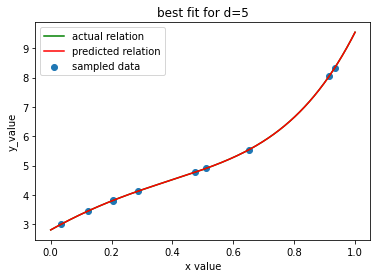
\includegraphics[width=10cm]{homework/homework_1/plot_1_1.png}
    \item this plot show that using $d=5$ we can find a $\hat{b}$ which perfectly estimate $g(X)$
    
    \end{itemize}

    
    
    \item (1 Points) Now you can adjust $d$. What is the minimum value for which we get a ``perfect fit"? How does this result relates with your conclusions on the approximation error above? 
    \begin{itemize}
    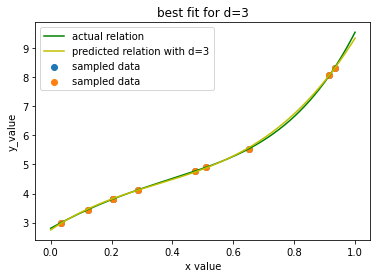
\includegraphics[width=10cm]{homework/homework_1/plot_1_2.png}
            \item this plot show that we can find very very close to the same relationship using $d=3$. this contrast with our conclusion above which was that we could model $g(x)$ perfectly with a degree 2 polynomial. The difference however is that in this case we were only allowing our model to learn from 10 data points. presumably if we increased the number of points to learn from we could reduce this number farther
    \end{itemize}
    
\setcounter{saveenum}{\value{enumi}}    
\end{enumerate}    

\textbf{\color{nyupurple} In presence of noise (13 Points)}\\
Now we will modify the true underlying $P_{\mathcal{X} \times \mathcal{Y}}$, adding some noise in $y = g(x) + \epsilon$, with $\epsilon \sim \gN(0,1)$ a standard normal random variable independent from $x$. We will call training error $e_t$ the empirical risk on the train set and generalization error $e_g$ the empirical risk on the test set.
\
\begin{enumerate}
\setcounter{enumi}{\value{saveenum}}

    \item (6 Points) Plot $e_t$ and $e_g$ as a function of $N$ for $d < N < 1000$ for $d = 2$, $d=5$ and $d=10$ (Plot 2). You may want to use a logarithmic scale in the plot. Include also plots similar to Plot 1 for 2 or 3 different values of $N$ for each value of $d$. 
    \begin{itemize}
    \item the code used to generate the bellow plots is here. 
            \item \inputminted[firstline=124, lastline=170, breaklines=True]{python}{hw1_code_source.py}
        \item 
             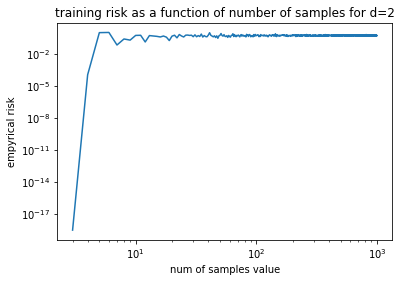
\includegraphics[width=5cm]{homework/homework_1/training_d_2.png}
            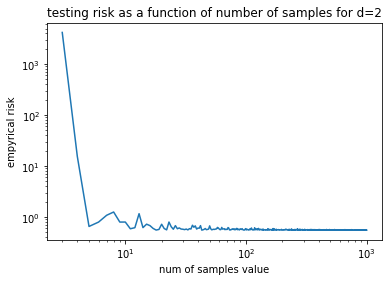
\includegraphics[width=5cm]{homework/homework_1/test_d_2.png}
             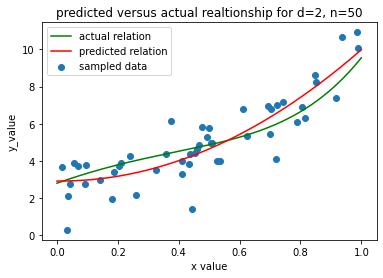
\includegraphics[width=5cm]{homework/homework_1/d_2_1.png}
             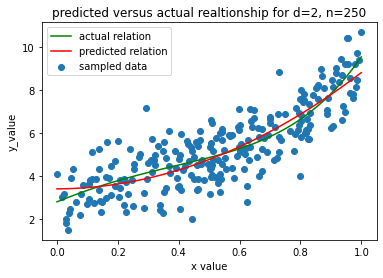
\includegraphics[width=5cm]{homework/homework_1/d_2_2.png}
            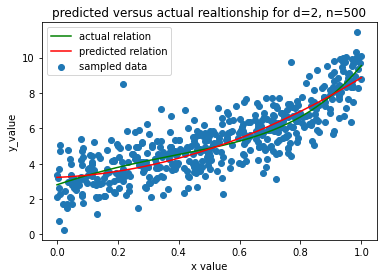
\includegraphics[width=5cm]{homework/homework_1/d_2_3.png}
            
              \item          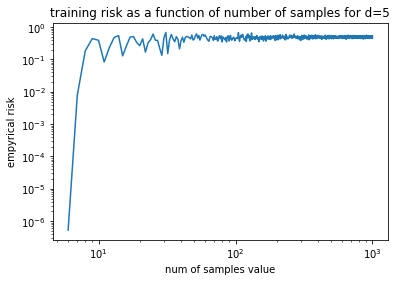
\includegraphics[width=5cm]{homework/homework_1/training_d_5.png}
            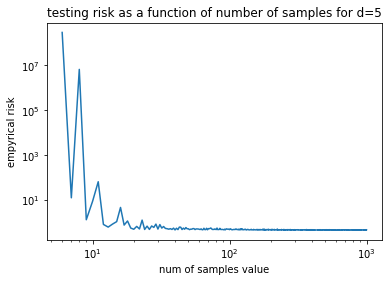
\includegraphics[width=5cm]{homework/homework_1/test_d_5.png}
             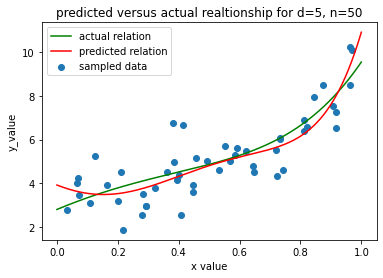
\includegraphics[width=5cm]{homework/homework_1/d_5_1.png}
             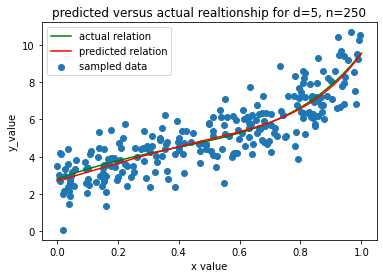
\includegraphics[width=5cm]{homework/homework_1/d_5_2.png}
            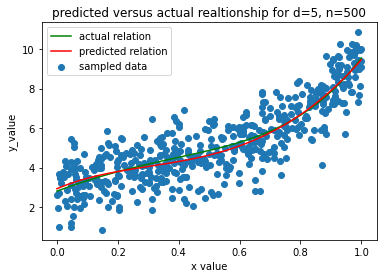
\includegraphics[width=5cm]{homework/homework_1/d_5_3.png}
            \item
                        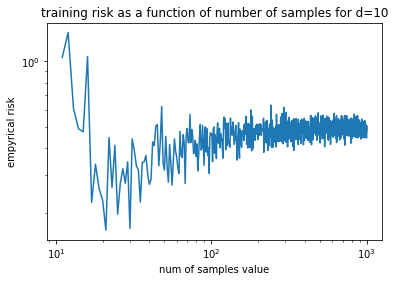
\includegraphics[width=5cm]{homework/homework_1/training_d_10.png}
            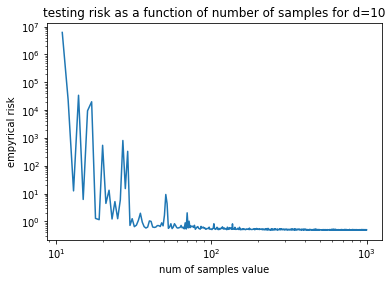
\includegraphics[width=5cm]{homework/homework_1/testing_d_10.png}
             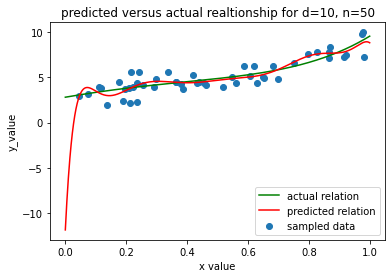
\includegraphics[width=5cm]{homework/homework_1/d_10_1.png}
             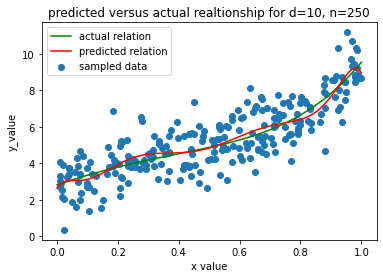
\includegraphics[width=5cm]{homework/homework_1/d_10_2.png}
            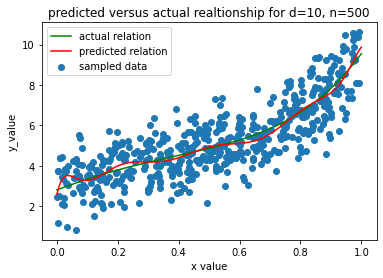
\includegraphics[width=5cm]{homework/homework_1/d_10_3.png}
    \item across all d values we can see that training error tends to increase for a period of time in n, this makes sense as a small number of points can be perfectly fit, but as more points are added the effect of noise in our sampling leads to training error. eventually however the increase in training error levels off presumably around the amount caused by noise in the data 
    \item testing error on the other hand across all values of d has an initial large drop off in testing error as n increases this makes sense as the data used to train the model is becoming more representative of the underlying population, the testing error eventually plateaus again presumably around the level of noise in the data. 
    \item  we can in general the the data does a poor job approximating the actual relationship with low levels of n but does better as n goes up. 
    \item it seems like d=2 under fits the relationship at low levels of n, and d=10 over fits the data at low levels of n which makes sense since the real data has dimension d=5
    
    \end{itemize}

    \item (4 Points) Recall the definition of the estimation error. Using the test set, (which we intentionally chose large so as to take advantage of the law of large numbers) give an empirical estimator of the estimation error. For the same values of $N$ and $d$ above plot the estimation error as a function of $N$ (Plot 3).
    \begin{itemize}
    \item i defined the empirical estimator of estimation error as    
            \item \inputminted[firstline=78, lastline=79, breaklines=True]{python}{hw1_code_source.py}
            \item where b is the minimum mean squared error estimator fit using just the training data, and super b is the minimum mean squared error estimator using the testing data. 
            \item i think this is a logical approach we are comparing the risk of super b which perfectly fits which is the best fit we could have for our testing error, with the risk of the best function we have found using our training set. 
        \item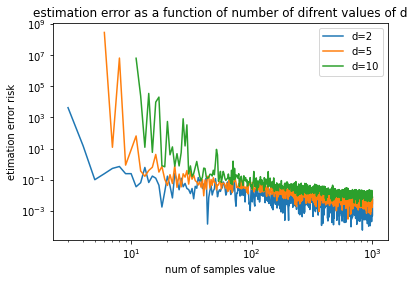
\includegraphics[width=10cm]{homework/homework_1/estimation_2.png}
        \item here we can see that overall empyrical estimation error goes down as n increases, which is logical as the training set is getting larger and generalization is getting better. 
        \item this decrease of course Plautus somewhere around the level of noise in the the testing set
        \item further it seems that lower values of d have lower testing errors, which makes sense since higher value of d models, require more parameters be fit with the same amount of data. 
    \end{itemize}
    \item (2 Points) The generalization error gives in practice an information related to the estimation error. Comment on the results of (Plot 2 and 3). What is the effect of increasing $N$? What is the effect of increasing $d$?
    \begin{itemize}
           \item we can see that for all values of d estimation error is decreasing in n. 
             \item we can see that estimation error eventually plateaus, this makes sense because we are estimating fixed parameters from data with noise so there is some level of ineducable error
             \item we can see that higher values of d have higher estimation error and take a larger n to stabilize this makes sense as for higher degree polynomials both noise is propagated and we are using the same amount of data to predict more parameters 
             \item so a higher n will lead to lower estimation error, and a higher d will lead to higher approximation error. 
    \end{itemize}
    
    \item (1 Points) Besides from the approximation and estimation there is a last source of error we have not discussed here. Can you comment on the optimization error of the algorithm we are implementing?
    \begin{itemize}
        \item this is a linear regression problem with a known closed form, so i don't think there is any numeric approximation going on (outside of maybe while inverting matrices) thus optimization error should be frailly minimal 
    \end{itemize}
\setcounter{saveenum}{\value{enumi}}    
\end{enumerate}

\textbf{\color{nyupurple} Application to Ozone data (optional) (2 Points)}\\
You can now use the code we developed on the synthetic example on a real world dataset. Using the command \texttt{np.loadtxt(`ozone\_wind.data')} load the data in the \emph{.zip}. The first column corresponds to ozone measurements and the second to wind measurements. You can try polynomial fits of the ozone values as a function of the wind values. 

\begin{enumerate}
\setcounter{enumi}{\value{saveenum}}
    \item (2 Points) Reporting plots, discuss the again in this context the results when varying $N$ (subsampling the training data) and $d$. 
\begin{itemize}
\item   here is my train test split code 
\item \inputminted[firstline=197, lastline=203, breaklines=True]{python}{hw1_code_source.py}

\\
    \item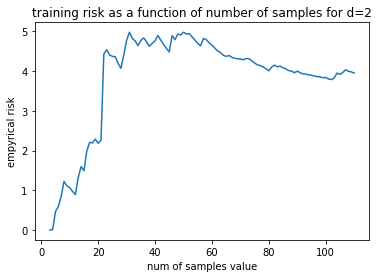
\includegraphics[width=5cm]{homework/homework_1/training_1.png}
    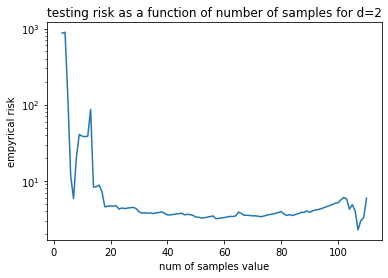
\includegraphics[width=5cm]{homework/homework_1/testing_1.png}
    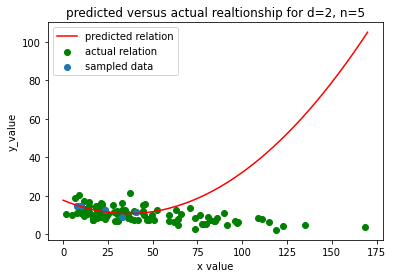
\includegraphics[width=5cm]{homework/homework_1/1_1.png}
    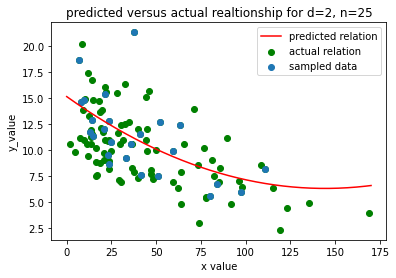
\includegraphics[width=5cm]{homework/homework_1/1_2.png}
    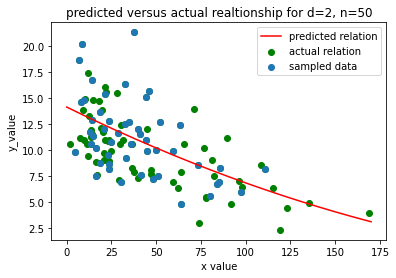
\includegraphics[width=5cm]{homework/homework_1/1_3.png}
        \item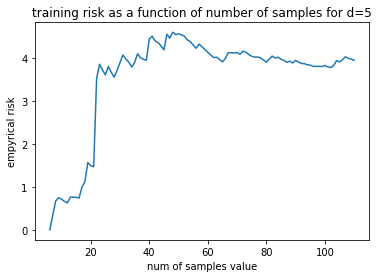
\includegraphics[width=5cm]{homework/homework_1/training_2.png}
    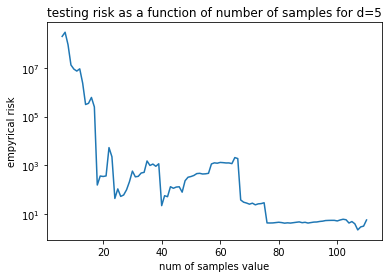
\includegraphics[width=5cm]{homework/homework_1/testing_2.png}
    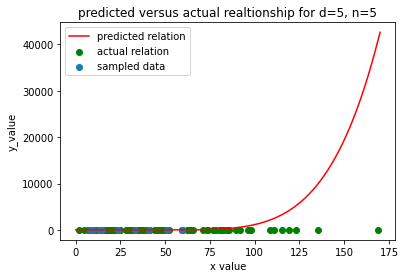
\includegraphics[width=5cm]{homework/homework_1/2_1.png}
    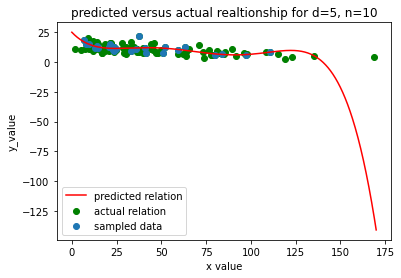
\includegraphics[width=5cm]{homework/homework_1/2_2.png}
    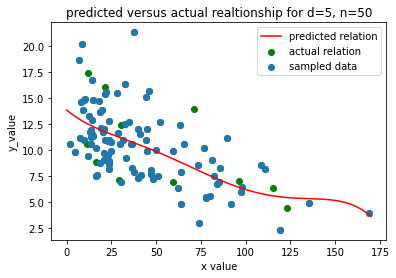
\includegraphics[width=5cm]{homework/homework_1/2_3.png}
        \item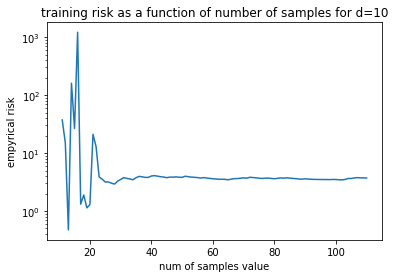
\includegraphics[width=5cm]{homework/homework_1/training_3.png}
    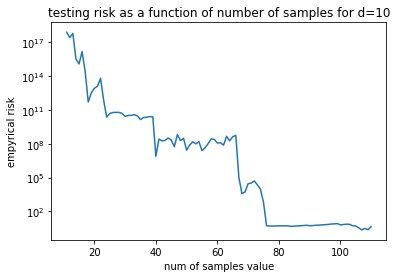
\includegraphics[width=5cm]{homework/homework_1/testing_3.png}
    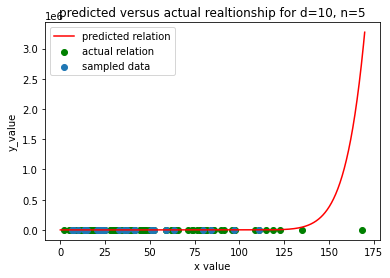
\includegraphics[width=5cm]{homework/homework_1/3_1.png}
    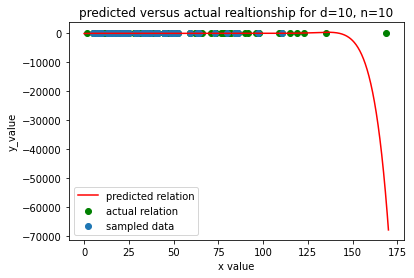
\includegraphics[width=5cm]{homework/homework_1/3_2.png}
    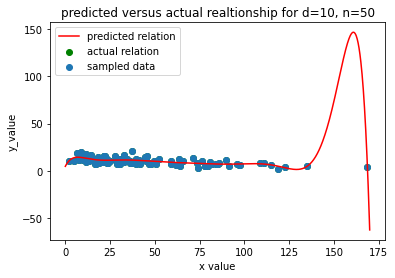
\includegraphics[width=5cm]{homework/homework_1/3_3.png}
    \item we can see that for all values of d as n increases training error initially spikes, and then stabilizes around a certain value. this makes sense as it easy to achieve low training error on a few points regardless of noise, but as the number of points in the training set go up there needs the noise is observed in the training error
    \item testing error on the other hand initially decreases in n and then stabilizes. This makes sense, as when $b$ is trained on only a few points, it will generalize well but as n goes up the model is more able to generalize, until it plateaus around the level of risk that comes from noise
    \item looking at d it seems that d=2 under fits the training data, and d=10 over fits the training data, so perhaps the degree of the polynomial is close to 5.
    \item this is all consistent with what we observed above
\end{itemize}
\end{enumerate}

\end{document}